\documentclass[t]{beamer}
\usetheme[deutsch]{KIT}
\setbeamercovered{transparent}
\setbeamertemplate{navigation symbols}{}

\KITfoot{Tutoriumsmaterial von Alexander Kwiatkowski, Michael Vollmer und Matthias Holoch \hspace{2.5cm} Basierend auf den Folien von Simon Stroh und Moritz v. Looz}
\usepackage[utf8]{inputenc}
\usepackage{amsmath}
\usepackage{ifthen}
\usepackage{amssymb}
\usepackage{tikz}
\usepackage{ngerman}
\usepackage[normalem]{ulem}
\usetikzlibrary{automata}
\usenavigationsymbols


\title{Theoretische Grundlagen der Informatik}
\subtitle{Tutorium}
\author{Alexander Kwiatkowski, Michael Vollmer und Matthias Holoch}

\institute[IKS]{Institut für Kryptographie und Sicherheit}

\TitleImage[height=\titleimageht]{images/tmaschine.png}

\newcommand{\N}{\ensuremath{\mathbb{N}}}
\newcommand{\M}{\ensuremath{\mathcal{M}}}
\newcommand{\classP}{\ensuremath{\mathcal{P}}}
\newcommand{\classNP}{\ensuremath{\mathcal{NP}}}
\newcommand{\co}{\ensuremath{\mathsf{co\text{-}}}}
\newcommand{\pot}{\ensuremath{\mathcal{P}}}
\newcommand{\abs}[1]{\ensuremath{\left\vert #1 \right\vert}}
\newcommand{\menge}[2]{\ensuremath{\left\lbrace #1 \,\middle\vert\, #2 \right\rbrace}}
\newcommand{\ducttape}[1]{\vspace{#1}}
\newcommand{\neglit}[1]{\overline{#1\vphantom{x^a}}}
\newcommand{\recipe}{\raisebox{-.3cm}{
\includegraphics[scale=.15]{images/chefs-cap.png}}\hspace{0.2cm}}
\newcommand{\opt}[1]{\ensuremath{\text{OPT}(#1)}}
\newcommand{\A}[1]{\ensuremath{\mathcal{A}(#1)}}
\renewcommand{\O}[1]{\ensuremath{\mathcal{O}(#1)}}
\newcommand{\msout}[1]{\text{\sout{\ensuremath{#1}}}}

\newcommand{\invincible}{\setbeamercovered{invisible}} %  "Yesss! I am invincible!!" (Boris Grishenko)
\newcommand{\vincible}{\setbeamercovered{transparent}}
\renewcommand{\solution}[1]{\invincible \pause #1 \vincible}
\newcommand{\micropause}{\\[8pt]}

% \@ifundefined{tikzset}{}{\tikzset{initial text=}} % Text "start" bei Startknoten unterdrücken
\tikzstyle{every node}=[thick]
\tikzstyle{every line}=[thick]

\newcommand{\tutnr}[1]{
  \subtitle{Tutorium #1}
	\begin{frame}
		\maketitle
	\end{frame}
}

\newcommand{\uebnr}[1]{
  \subtitle{Anmerkungen zum #1. Übungsblatt}
	\begin{frame}
		\maketitle
	\end{frame}
}

\begin{document}

\newcommand{\start}[3]
{
  \draw (#1*2,#2*2) node{$#3$};
  \draw (#1*2,#2*2) circle(0.4cm);
  \draw [->] (#1*2-0.9,#2) -- (#1*2-0.4,#2);
}
\newcommand{\final}[3]
{
  \draw (#1*2,#2*2) node{$#3$};
  \draw (#1*2,#2*2) circle(0.4cm);
  \draw (#1*2,#2*2) circle(0.32cm);
}
\newcommand{\startfinal}[3]
{
  \draw (#1*2,#2*2) node{$#3$};
  \draw (#1*2,#2*2) circle(0.4cm);
  \draw (#1*2,#2*2) circle(0.32cm);
  \draw [->] (#1*2-0.9,#2) -- (#1*2-0.4,#2);
}
\newcommand{\state}[3]
{
  \draw (#1*2,#2*2) node{$#3$};
  \draw (#1*2,#2*2) circle(0.4cm);
}
\newcommand{\tol}[4]
{
  \draw (#1+#3,#2*2) node[above]{$#4$};
  \draw [->] (#1*2-0.4,#2*2) -- (#3*2+0.4,#2*2);
}
\newcommand{\tor}[4]
{
  \draw (#1+#3,#2*2) node[above]{$#4$};
  \draw [->] (#1*2+0.4,#2*2) -- (#3*2-0.4,#2*2);
}
\newcommand{\tot}[4]
{
  \draw (#1*2,#2+#3) node[right]{$#4$};
  \draw [->] (#1*2,#2*2+0.4) -- (#1*2,#3*2-0.4);
}
\newcommand{\tob}[4]
{
  \draw (#1*2,#2+#3) node[right]{$#4$};
  \draw [->] (#1*2,#2*2-0.4) -- (#1*2,#3*2+0.4);
}
\newcommand{\totl}[5]
{
  \draw (#1+#3,#2+#4) node[above right]{$#5$};
  \draw [->] (#1*2-0.283,#2*2+0.283) -- (#3*2+0.283,#4*2-0.283);
}
\newcommand{\totr}[5]
{
  \draw (#1+#3,#2+#4) node[above left]{$#5$};
  \draw [->] (#1*2+0.283,#2*2+0.283) -- (#3*2-0.283,#4*2-0.283);
}
\newcommand{\tobl}[5]
{
  \draw (#1+#3,#2+#4) node[below right]{$#5$};
  \draw [->] (#1*2-0.283,#2*2-0.283) -- (#3*2+0.283,#4*2+0.283);
}
\newcommand{\tobr}[5]
{
  \draw (#1+#3,#2+#4) node[below left]{$#5$};
  \draw [->] (#1*2+0.283,#2*2-0.283) -- (#3*2-0.283,#4*2+0.283);
}
\newcommand{\rloopl}[3]
{
  \draw (#1*2-1,#2*2) node[left]{$#3$};
  \draw [->] (#1*2-0.35,#2*2-0.2) arc (-30:-320:0.32cm);
}
\newcommand{\rloopr}[3]
{
  \draw (#1*2+1,#2*2) node[right]{$#3$};
  \draw [->] (#1*2+0.35,#2*2+0.2) arc (150:-140:0.32cm);
}
\newcommand{\rloopt}[3]
{
  \draw (#1*2,#2*2+1) node[above]{$#3$};
  \draw [->] (#1*2-0.2,#2*2+0.35) arc (240:-50:0.32cm);
}
\newcommand{\rloopb}[3]
{
  \draw (#1*2,#2*2-1) node[below]{$#3$};
  \draw [->] (#1*2+0.2,#2*2-0.35) arc (60:-230:0.32cm);
}
\newcommand{\lloopl}[3]
{
  \draw (#1*2-1,#2*2) node[left]{$#3$};
  \draw [->] (#1*2-0.35,#2*2+0.2) arc (30:320:0.32cm);
}
\newcommand{\lloopr}[3]
{
  \draw (#1*2+1,#2*2) node[right]{$#3$};
  \draw [->] (#1*2+0.35,#2*2-0.2) arc (-150:140:0.32cm);
}
\newcommand{\lloopt}[3]
{
  \draw (#1*2,#2*2+1) node[above]{$#3$};
  \draw [->] (#1*2+0.2,#2*2+0.35) arc (-60:230:0.32cm);
}
\newcommand{\lloopb}[3]
{
  \draw (#1*2,#2*2-1) node[below]{$#3$};
  \draw [->] (#1*2-0.2,#2*2-0.35) arc (-240:50:0.32cm);
}
\tutnr{4}

\section{Altlasten}
\subsection{Pumping Lemma}
\begin{frame}
	\frametitle{Pumping Lemma Formalia}

\end{frame}

\subsection{Chomsky-Normalform}
\frame{
\frametitle{Chomsky-Normalform}
}

\section{CYK-Algorithmus}
\subsection{CYK-Algorithmus}
\frame{
\frametitle{CYK Überblick}
CYK ist ein Algorithmus, um das Wortproblem in CH-2 zu lösen. Um den Algorithmus anzuwenden, muss eine Grammatik in Chomsky-Normalform vorliegen.\\
Grundidee zur Überprüfung eines Wortes der Länge $n$:
\begin{itemize}
\item Wir betrachen $V_{i,j} = $ Menge der Nichtterminale, aus denen das Teilwort der Position $i$ bis $j$ abgeleitet werden kann
\item Die Frage, ob $V_{i,j}$ ableitbar ist, lässt sich entscheiden durch Betrachten aller möglichen $V_{i,k}$ und $V_{k+1,j}$
\item $V_{i,i}$ sind trivial
\item Bottom-up lässt sich dadurch $V_{1,n}$ berechnen
\item Ist $S \in V_{1,n}$, so lässt sich das Wort ableiten
\end{itemize}
}

\frame{
\frametitle{CYK Beispiel}
Gegeben sei die Grammatik \textit{G} $= \mathcal{(T,V,}S\mathcal{,P) }$  mit den folgenden Produktionen aus $\mathcal{P}$:
\begin{align*}
S & \rightarrow AX \mid AB \\
X &\rightarrow SB \mid AB \\
A &\rightarrow a\\
B &\rightarrow b\\
\end{align*}
\begin{enumerate}
	\item Lässt sich der CYK-Algorithmus auf $G$ anwenden?
	\item Ist das Wort $aaabbb$ in der Sprache $\mathcal{L}(\textit{G})$?
\end{enumerate}
}

\subsection{Alte Aufgabe 2b}
\begin{frame}
	\frametitle{Alte Aufgabe 2 Fortsetzung}
	Gegeben sei die folgende Grammatik: $\mathcal{G} = (\mathcal{T},\mathcal{V},S,
	\mathcal{P})$ mit\\
	$\mathcal{T} := \{a,b,c,d\}$, $\mathcal{V} := \{S,A,D,M\}$, $\mathcal{P} := \{
	S \rightarrow AMD \; | \; M, A \rightarrow AA \; | \; a, D \rightarrow DD \; | \; d,
	M \rightarrow bMc \; | \; \lambda\}$
	\begin{enumerate}
		\item Geben Sie die erzeugte Sprache an!
		\item Wandeln Sie die gegebene kontextfreie Grammatik $\mathcal{G}$ in eine
		"aquivalente kontextfreie Grammatik $\mathcal{G}'$ in\\
		Chomsky-Normalform um, indem sie jeden Schritt durch eine neue Grammatik beschreiben!
		\item Zeigen oder widerlegen Sie mit Hilfe des CYK-Algorithmus, ob die folgenden
		W"orter in der Sprache $\mathcal{L}$\\
		liegen, die durch die Grammatik $\mathcal{G}$ erzeugt wird!
		\begin{enumerate}
			\item $aabbccdd$
			\item $abbcc$
			\item $abcdd$
		\end{enumerate}
	\end{enumerate}
\end{frame}

\section{Kellerautomaten}
\subsection{Kellerautomaten}
\begin{frame}
	\frametitle{Definition Kellerautomaten}
	Ein (nichtdeterministischer) \textbf{Kellerautomat} (NPDA bzw PDA, Pushdown Automaton) besteht aus $(Q, \Sigma, \Gamma, q_0, Z_0,\delta, F)$, wobei
	\begin{itemize}
		\item $Q$ endliche Zustandsmenge
		\item $\Sigma$ endliches Eingabealphabet
		\item $\Gamma$ endliches Stack-Alphabet
		\item $q_0 \in Q$ Anfangszustand
		\item $Z_0 \in \Gamma$ Initialisierung des Stacks
		\item $\delta : Q \times ( \Sigma \cup \{\lambda\}) \times \Gamma \rightarrow 2^{Q \times \Gamma^*}$
		\begin{itemize}
			\item $\delta(q, a, Z) \subseteq \{(q,\gamma) : q \in Q, \gamma \in \Gamma^*\}$
			\item $\delta(q, \lambda, Z) \subseteq \{(q,\gamma) : q \in Q, \gamma \in \Gamma^*\}$
		\end{itemize}
		\item $F \subseteq Q$ Menge der akzeptierenden Endzustände, $F=\emptyset$ ist möglich.
		
		\vspace{-4cm}\raggedleft{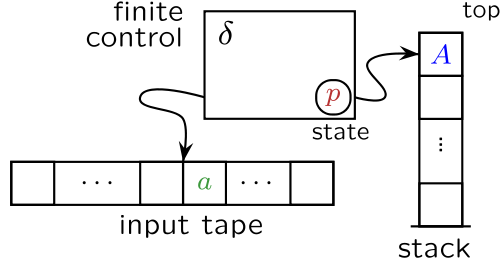
\includegraphics[width=0.5\textwidth]{images/PDA.png}}
	\end{itemize}
\end{frame}

\begin{frame}
\frametitle{Zu Kellerautomaten}
\begin{itemize}
\item Akzeptieren nach Eingabeende, wenn \begin{itemize}
	\item der Stack leer ist \emph{oder}
	\item der Automat in einen akzeptierenden Zustand kommt.
\end{itemize}
\item Sind im Allgemeinen nichtdeterministisch
\item Man kann Endzustände auch aus der Definition weglassen und alternativ verlangen, dass der Automat genau bei leerem Keller akzeptiert.
\item Man kann sogar alle Zustände bis auf einen weglassen und alles in die Kellerbelegung kodieren
\end{itemize}
\end{frame}

\begin{frame}
	\frametitle{Beispiel}
	$M = (Q, \Sigma, \Gamma, q_0, Z_0, \delta, F)$
	\begin{itemize}
		\item $Q = \{q_0, q_1, q_2\}$
		\item $\Sigma = \{a,b\}$
		\item $\Gamma = \{\#,X\}$
		\item $Z_0 = \#$
		\item $F = \{q_2\}$
	\end{itemize}
	\begin{figure}
		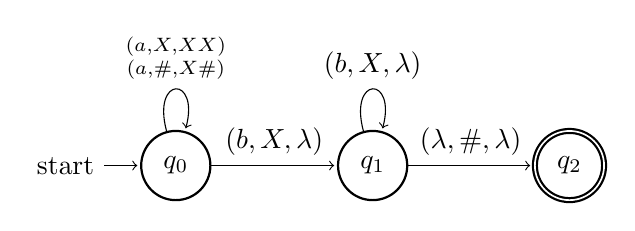
\begin{tikzpicture}[node distance=2.5cm,shorten >=1pt,auto]
			\node[state,initial]   (q_0)                {$q_0$};
			\node[state]           (q_1) [right of=q_0] {$q_1$};
			\node[state,accepting] (q_2) [right of=q_1] {$q_2$};
			\path[->]	(q_0) 	edge 			node {$(b,X,\lambda)$}				(q_1)
			edge [loop above]	node {${(a,X,XX)} \atop {(a,\#,X\#)}$}	 	()
			(q_1)	edge			node {$(\lambda,\#,\lambda)$}			(q_2)
			edge [loop above]	node {$(b,X,\lambda)$}				();
		\end{tikzpicture}
	\end{figure}
	\begin{itemize}
		\item Welche Sprache akzeptiert dieser Automat?
	\end{itemize}
\end{frame}

\subsection{Alte Aufgabe 3}
\begin{frame}
	\frametitle{Alte Aufgabe 3}
	Gegeben sei folgende Sprache f"ur das Alphabet $\Sigma = \{a,b,c\}$:
	\begin{multline*}
		\mathcal{L} = \{w_1w_2 \in \Sigma^* \; | \; w_1 \in \{a,b\}^*,w_2 \in \{b,c\}^*,\\
		\#_a w_1 + \#_b w_1 = \#_b w_2 + \#_c w_2\}
	\end{multline*}
	Hier gibt $\#_x w$ die H"aufigkeit des Vorkommens eines Zeichens $x \in \Sigma$ in
	einem Wort $w \in \Sigma^*$ an.
	\begin{enumerate}
		\item Zeigen Sie, dass $\mathcal{L}$ nicht regul"ar ist!
		\item Geben Sie eine Chomsky-2-Grammatik an, die genau die Sprache $\mathcal{L}$
		erzeugt!
		\item Geben Sie einen Kellerautomaten $\mathcal{M}$ an, der genau die Sprache
		$\mathcal{L}$ erkennt! Zeichnen Sie den\\
		Zustands"ubergangsgraphen f"ur $\mathcal{M}$!
	\end{enumerate}
\end{frame}

\subsection{Pumping Lemma für kontextfreie Sprachen}
\begin{frame}
	\frametitle{Pumping-Lemma für kontextfreie Sprachen}
	\begin{exampleblock}{Lemma}
		Für jede kontextfreie Sprache $L$ gibt es eine Konstante $n \in \mathbb{N}$,
		so dass sich jedes Wort $z \in L$ mit $|z| \geq n$ so als
		$$ z = uvwxy $$
		schreiben lässt, dass
		\begin{itemize}
			\item $|vx| \geq 1$,
			\item $|vwx| \leq n$ und
			\item für alle $i \geq 0$ das Wort $uv^iwx^iy \in L$ ist.
		\end{itemize}
	\end{exampleblock}
\end{frame}

\begin{frame}
	\frametitle{Beweisidee}
	\begin{itemize}
		\item Jeder Knoten im Ableitungsbaum (wie wir ihn in CYK sehen) steht für ein Nichtterminalsymbol
		\item Ab einer gewissen Höhe des Baumes (bzw. Länge des Wortes) muss ein Nichtterminal im Baum mehrmals in einer Reihe vorkommen
		\item Man kann also aus einem Nichtterminalsymbol dasselbe Symbol wieder ableiten
		\item Da das Wort durch jede Ableitung (außer zu Terminalsymbolen) länger wird, gibt es eine "`Schleife"' beim Ableiten
		\item Diese Schleife kann man also "`pumpen"', also beliebig oft (oder auch gar nicht) durchlaufen
	\end{itemize}
\end{frame}

\begin{frame}
	\frametitle{Beweisidee}
	\begin{figure}[H]
		\centering
		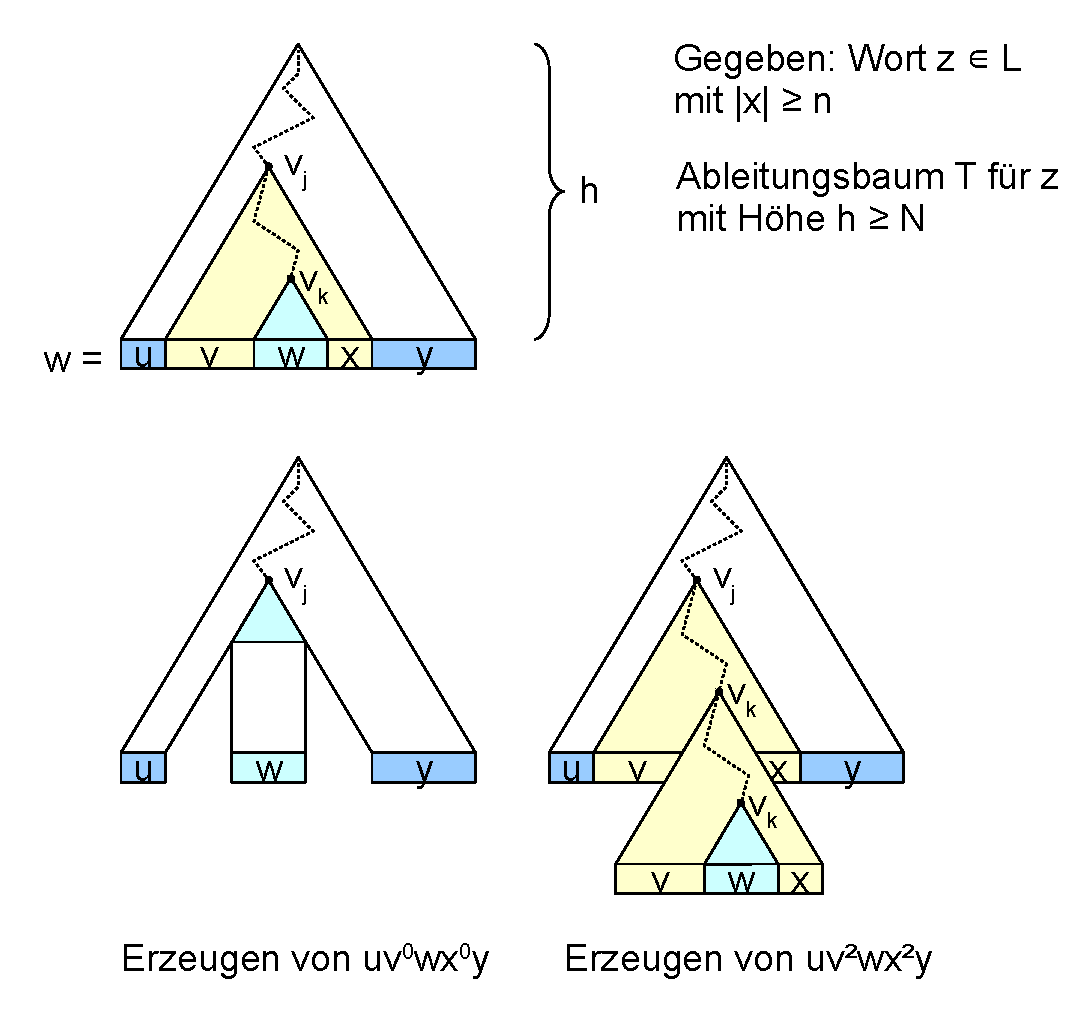
\includegraphics[scale=0.5]{images/pumping}
	\end{figure}
\end{frame}

\subsection{Aufgabe 1}
\begin{frame}
	\frametitle{Aufgabe 1}
	\begin{enumerate}
		\item Geben Sie f"ur die Sprache $\mathcal{L} = \{a^nb^nc^n \; | \; n \in
		\mathbb{N}\}$ eine Grammatik des h"ochstm"oglichen Chomsky-Typs an!
		\item Zeigen Sie, dass die Sprache $\mathcal{L}' = \{a^{2^n} \; | \; n \in
		\mathbb{N}\}$ nicht kontextfrei ist!
	\end{enumerate}
\end{frame}

\section{Schluss}
\subsection{Schluss}

\begin{frame}
\frametitle{Bis zum nächsten Mal!}
\begin{center}
  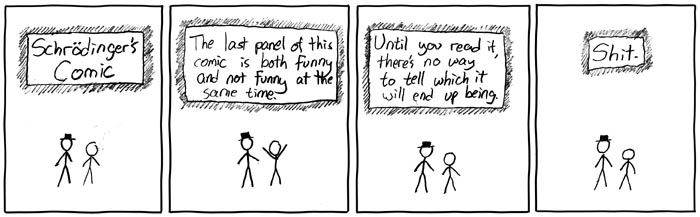
\includegraphics[width=1.5 \textheight]{images/schrodinger.jpg}
\end{center}
\end{frame}

\frame{
  \frametitle{Lizenzen}
  \center
  
\includegraphics[width=2em]{images/by}
  
\includegraphics[width=2em]{images/cc}
  
\includegraphics[width=2em]{images/sa}
  \\
  {\tiny

Dieses Werk ist unter einem ``Creative Commons Namensnennung-Weitergabe unter gleichen Bedingungen 3.0 Deutschland``-Lizenzvertrag lizenziert. Um eine Kopie der Lizenz zu erhalten, gehen Sie bitte zu \href{http://creativecommons.org/licenses/by-sa/3.0/de/}{http://creativecommons.org/licenses/by-sa/3.0/de/} oder schreiben Sie an Creative Commons, 171 Second Street, Suite 300, San Francisco, California 94105, USA.\\
  \vspace{1cm}
  Davon ausgenommen sind das Titelbild, welches aus der März-April 2002 Ausgabe von American Scientist erschienen ist und ohne Erlaubnis verwendet wird, sowie das KIT Beamer Theme. Hierfür gelten die Bestimmungen der jeweiligen Urheber.
  \vspace{1cm}
  \\ 
  }
  %Habe hier die Reihenfolge etwas umgestellt, weil die Formatierung bei mir komisch aussah. 
  %Wenn es bei dir anders ist, kannst du es auch wieder zurückändern, dann haben wir unterschiedliche Kompilieroptionen
}

\end{document}